\documentclass[supercite]{Experimental_Report}

\title{~~~~~~新生实践课~~~~~~}
\author{王李超}
\school{计算机科学与技术学院}
\classnum{CS启明2401}
\stunum{U202414887}
\instructor{范晔斌} % 李平、孙伟平、范晔斌、陈加忠
\date{2024年12月1日}

\usepackage{algorithm, multirow}
\usepackage{algpseudocode}
\usepackage{amsmath}
\usepackage{amsthm}
\usepackage{framed}
\usepackage{mathtools}
\usepackage{subcaption}
\usepackage{xltxtra} %提供了针对XeTeX的改进并且加入了XeTeX的LOGO, 自动调用xunicode宏包(提供Unicode字符宏)
\usepackage{bm}
\usepackage{tikz}
\usepackage{tikzscale}
\usepackage{pgfplots}
%\usepackage{enumerate}

\pgfplotsset{compat=1.16}

\newcommand{\cfig}[3]{
  \begin{figure}[htb]
    \centering
    \includegraphics[width=#2\textwidth]{images/#1.tikz}
    \caption{#3}
    \label{fig:#1}
  \end{figure}
}

\newcommand{\sfig}[3]{
  \begin{subfigure}[b]{#2\textwidth}
    \includegraphics[width=\textwidth]{images/#1.tikz}
    \caption{#3}
    \label{fig:#1}
  \end{subfigure}
}

\newcommand{\xfig}[3]{
  \begin{figure}[htb]
    \centering
    #3
    \caption{#2}
    \label{fig:#1}
  \end{figure}
}

\newcommand{\rfig}[1]{\autoref{fig:#1}}
\newcommand{\ralg}[1]{\autoref{alg:#1}}
\newcommand{\rthm}[1]{\autoref{thm:#1}}
\newcommand{\rlem}[1]{\autoref{lem:#1}}
\newcommand{\reqn}[1]{\autoref{eqn:#1}}
\newcommand{\rtbl}[1]{\autoref{tbl:#1}}

\algnewcommand\Null{\textsc{null }}
\algnewcommand\algorithmicinput{\textbf{Input:}}
\algnewcommand\Input{\item[\algorithmicinput]}
\algnewcommand\algorithmicoutput{\textbf{Output:}}
\algnewcommand\Output{\item[\algorithmicoutput]}
\algnewcommand\algorithmicbreak{\textbf{break}}
\algnewcommand\Break{\algorithmicbreak}
\algnewcommand\algorithmiccontinue{\textbf{continue}}
\algnewcommand\Continue{\algorithmiccontinue}
\algnewcommand{\LeftCom}[1]{\State $\triangleright$ #1}

\newtheorem{thm}{定理}[section]
\newtheorem{lem}{引理}[section]

\colorlet{shadecolor}{black!15}

\theoremstyle{definition}
\newtheorem{alg}{算法}[section]

\def\thmautorefname~#1\null{定理~#1~\null}
\def\lemautorefname~#1\null{引理~#1~\null}
\def\algautorefname~#1\null{算法~#1~\null}

\begin{document}

\maketitle

\clearpage

\pagenumbering{Roman}

\tableofcontents[level=2]
\clearpage

\pagenumbering{arabic}

\section{网页整体框架}

图\ref{fig1-1}这个网页的整体框架使用HTML与CSS实现,结构清晰简洁,包含头部、主体内容和底部三个主要部分。头部部分通过`<header>`标签呈现,显示网站标题“王李超的个人主页”,背景为黑色半透明,文字居中,视觉效果突出。主体内容区域由一个`<div>`容器构成,采用Flexbox布局,使内容水平居中对齐,容器内放置了五个链接盒子,分别通向“个人经历”“喜欢的音乐”“我的Steam”“Github主页”和“我的资源”页面。每个链接盒子有独特的背景图、文字说明,并添加了悬停时的动画效果,如放大、阴影变化及模糊背景图变清晰,提升交互体验。底部区域由`<footer>`标签定义,显示欢迎语和简单介绍,同样采用黑色半透明背景,使整体风格一致。整个页面的布局通过CSS控制,使网页在不同屏幕设备上自适应,从而提供良好的用户体验,整体风格现代、简洁而不失个性。
% \begin{enumerate}
% \renewcommand{\labelenumi}{\theenumi)}
% 	\item C++
% 	\item Java
% 	\item HTML
% \end{enumerate}

\begin{figure}[htb] % here top bottom
	\begin{center}
		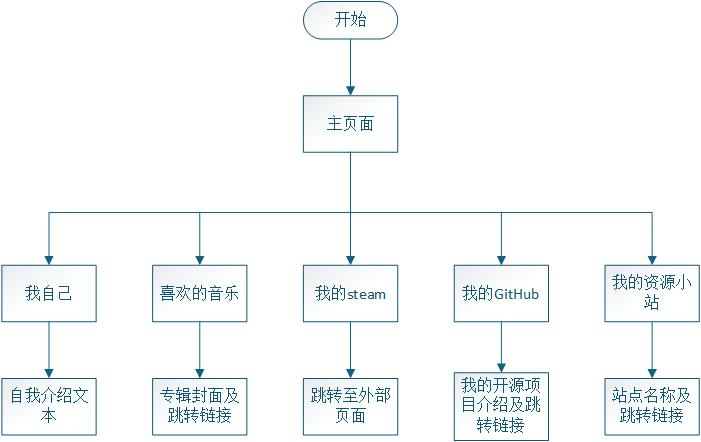
\includegraphics[scale=0.80]{images/1-1.jpg}
		\caption{网页整体框架举例}
		\label{fig1-1}
	\end{center}
\end{figure}

\newpage

\section{主页设计}

1. 头部结构:头部区域使用`<header>`标签,显示网页标题“王李超的个人主页”,文字居中,采用白色字体和黑色透明背景。此设计增加了标题的视觉层次感,同时保持整体简洁大方。

2. 主体内容布局:主体区域通过一个`<div class="content">`容器承载,主要功能是展示五个链接盒子。每个盒子分别对应“个人经历”“喜欢的音乐”“我的Steam”“Github主页”和“我的资源”五个子页面,链接直观明了,方便导航。

3. 盒子设计:每个链接盒子都采用白色半透明背景,带有圆角和阴影效果。盒子内文字居中显示,使用粗体设计,整体呈现干净、现代的风格。盒子宽高比为黄金比例,使视觉效果更加和谐。

4. 动态交互效果:盒子设计中加入悬停时的动画效果,通过CSS实现。当鼠标悬停时,盒子会放大并增强阴影效果,同时背景图片从模糊变为清晰,使用户体验更加生动且有趣。

5. 布局实现:整个页面使用Flexbox布局,确保内容在不同设备和屏幕尺寸下都能保持良好的自适应效果。盒子排列居中,水平间距均匀,增强页面的对称性和美观度。

6. 底部结构:底部区域使用`<footer>`标签,展示欢迎信息和个人简介。采用黑色透明背景,与头部设计保持一致,文字居中排布,简洁而不失信息量。

7. 色彩与背景:页面整体以深色为主,通过透明背景与半透明盒子形成视觉对比。同时,页面背景为全屏图像,增加页面的层次感和视觉吸引力,使整体风格更具现代感。

8. 响应式设计:通过`<meta>`标签设置视口,使页面能自动适应各种设备屏幕尺寸,优化了移动设备的浏览体验,从而增强了网站的兼容性与实用性。

9. 设计思路总结:整个页面设计追求简洁、现代和互动性,突出用户体验。通过色彩、动画效果及布局优化,使用户在视觉和交互上都能感受到良好的体验。请见图\ref{fig2-1}。


\begin{figure}[htb]
	\begin{center}
		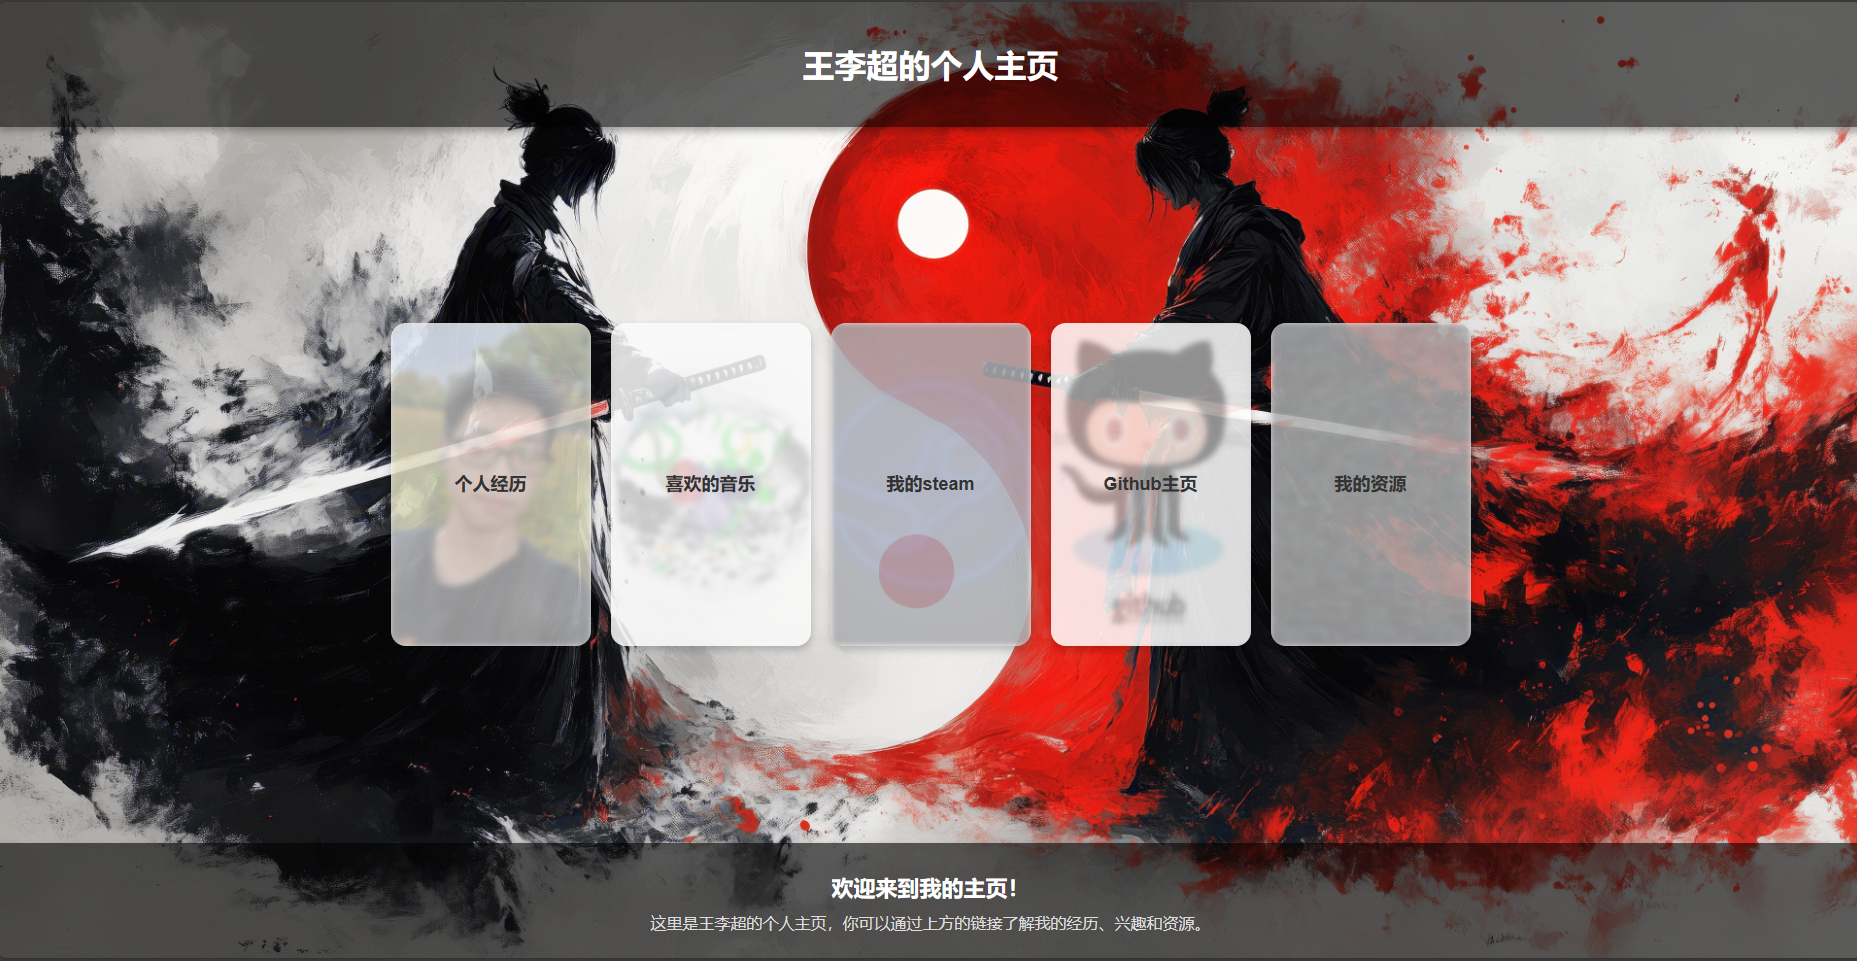
\includegraphics[scale=0.30]{images/2-1.png}
		\caption{主页举例}
		\label{fig2-1}
	\end{center}
\end{figure}

\newpage

\section{分页面设计}

\subsection{页面1 (个人信息页面设计)}

图\ref{fig3-1}该页面以展示“王李超的个人主页 - 个人资料”为主题,设计中遵循简洁、直观的原则,整体风格统一,易于用户浏览。页面头部使用\texttt{<header>}标签定义,标题“王李超的个人主页 - 个人资料”居中显示,采用黑色半透明背景与白色文字,形成简洁大方的视觉效果。通过适当的\texttt{padding},提升标题的可读性和整体页面的舒适感。主体部分通过\texttt{<div class="content">}容器包裹,采用Flexbox布局,使内容在垂直与水平方向居中对齐,确保在不同屏幕尺寸下依然保持居中状态。个人信息部分通过\texttt{<div class="project-details">}展示,每条信息单独使用\texttt{<div class="line">}包裹,增加白色字体与半透明背景,增强可读性和视觉层次感。每条信息块添加圆角、内边距及阴影效果,使用\texttt{box-shadow}提升立体感。此外,通过\texttt{white-space: nowrap}保证每段信息一行显示,使排版整洁。页面底部提供了跳转至Github的链接,用户点击即可访问相关资源。底部使用\texttt{<footer>}标签定义,背景风格与头部保持一致,采用黑色透明背景、白色文字,整体视觉风格和谐统一。通过\texttt{text-align: center}使欢迎信息与简要说明居中排列,进一步增强整体视觉的均衡感。为确保页面在各类设备上的适应性,通过\texttt{<meta>}视口设置,实现内容自适应布局。同时,Flexbox布局使各元素在不同屏幕尺寸下均保持居中,提高用户体验。文字内容设置最大宽度为视口宽度的100\%,防止内容溢出,提升排版稳定性。整体设计考虑了美观与实用性,确保在信息传递的同时,保持页面的简洁与高效。

\begin{figure}[htb]
	\begin{center}
		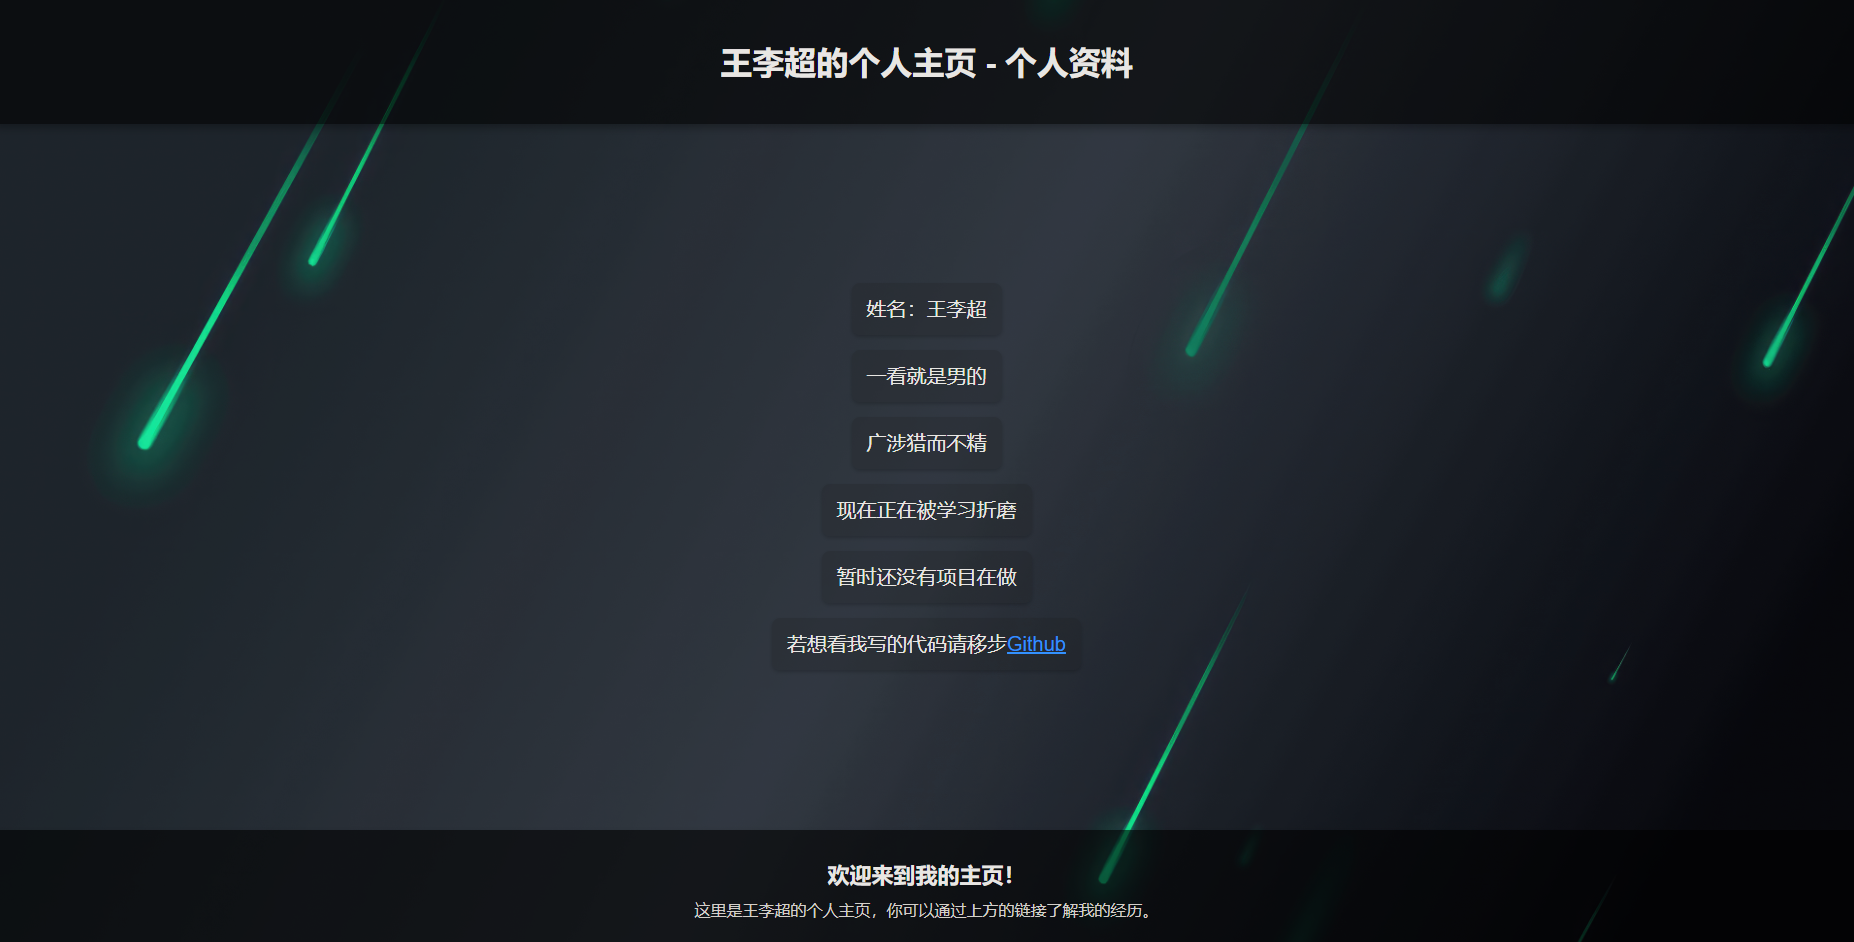
\includegraphics[scale=0.20]{images/3-1.png}
		\caption{分页面举例}
		\label{fig3-1}
	\end{center}
\end{figure}

\begin{shaded*}
	\begin{alg}{网页源代码}
		\label{alg:1}
		\begin{algorithmic}
			\State \textbf{<!DOCTYPE html>}
			\State \textbf{<html lang="zh-CN">}
			\State \ \ \ \ \textbf{<head>}
			\State \ \ \ \ \ \ \ \ \ \textbf{<meta charset="UTF-8">}
			\State \ \ \ \ \ \ \ \ \ \textbf{<meta name="viewport" content="width=device-width, initial-scale=1.0">}
			\State \ \ \ \ \ \ \ \ \ \textbf{<title>王李超的个人主页 - 个人资料</title>}
			\State \ \ \ \ \ \ \ \ \ \textbf{<link rel="icon" href="../images/favicon.ico" type="image/x-icon">}
			\State \ \ \ \ \ \ \ \ \ \textbf{<style>}
			\State \ \ \ \ \ \ \ \ \ \ \ \textbf{body \{} \texttt{font-family: Arial, sans-serif;}
			\State \ \ \ \ \ \ \ \ \ \ \ \ \textbf{background-image: url('experience\_background.png');}
			\State \ \ \ \ \ \ \ \ \ \ \ \ \textbf{background-size: cover;}
			\State \ \ \ \ \ \ \ \ \ \ \ \ \textbf{background-position: center;}
			\State \ \ \ \ \ \ \ \ \ \ \ \ \textbf{background-attachment: fixed;}
			\State \ \ \ \ \ \ \ \ \ \ \ \ \textbf{color: hsl(0, 0\%, 0\%); }
			\State \ \ \ \ \ \ \ \ \ \ \ \ \textbf{display: flex;}
			\State \ \ \ \ \ \ \ \ \ \ \ \ \textbf{flex-direction: column;}
			\State \ \ \ \ \ \ \ \ \ \ \ \ \textbf{min-height: 100vh;}
			\State \ \ \ \ \ \ \ \ \ \ \ \textbf{<style>}
			\State \ \ \ \ \textbf{<body>}
			\State \ \ \ \ \ \ \ \ \textbf{<header>}
			\State \ \ \ \ \ \ \ \ \ \ \ \textbf{<h1>王李超的个人主页 - 个人资料</h1>}
			\State \ \ \ \ \ \ \ \ \textbf{</header>}
			\State \ \ \ \ \ \ \ \ \textbf{<div class="content">}
			\State \ \ \ \ \ \ \ \ \ \ \ \textbf{<div class="project-details">}
			\State \ \ \ \ \ \ \ \ \ \ \ \ \textbf{<div class="line">姓名:王李超</div>}
			\State \ \ \ \ \ \ \ \ \ \ \ \ \textbf{<div class="line">一看就是男的</div>}
			\State \ \ \ \ \ \ \ \ \ \ \ \ \textbf{<div class="line">广涉猎而不精</div>}
			\State \ \ \ \ \ \ \ \ \ \ \ \ \textbf{<div class="line">现在正在被学习折磨</div>}
			\State \ \ \ \ \ \ \ \ \ \ \ \ \textbf{<div class="line">暂时还没有项目在做</div>}
			\State \ \ \ \ \ \ \ \ \ \ \ \ \textbf{<div class="line">若想看我写的代码请移步<a href="web/github.html">Github</a></div>}
			\State \ \ \ \ \ \ \ \ \ \ \ \textbf{</div>}
			\State \ \ \ \ \ \ \ \ \textbf{</div>}
			\State \ \ \ \ \ \ \ \ \textbf{<footer>}
			\State \ \ \ \ \ \ \ \ \ \ \ \textbf{<h2>欢迎来到我的主页!</h2>}
			\State \ \ \ \ \ \ \ \ \ \ \ \textbf{<p>这里是王李超的个人主页,你可以通过上方的链接了解我的经历。</p>}
			\State \ \ \ \ \ \ \ \ \textbf{</footer>}
			\State \textbf{</body>}
			\State \textbf{</html>}
		\end{algorithmic}
	\end{alg}
	\end{shaded*}
	

\subsection{喜欢的音乐}

图\ref{fig3-2}这部分内容与主页面非常相似,不同的是修改了三个方框的大小 和模糊程度,使文字更加清晰可见。修改方框大小主要是为了适应专辑封面一比一的比例,以及让页面看起来更充实。

\begin{figure}[htb]
	\begin{center}
		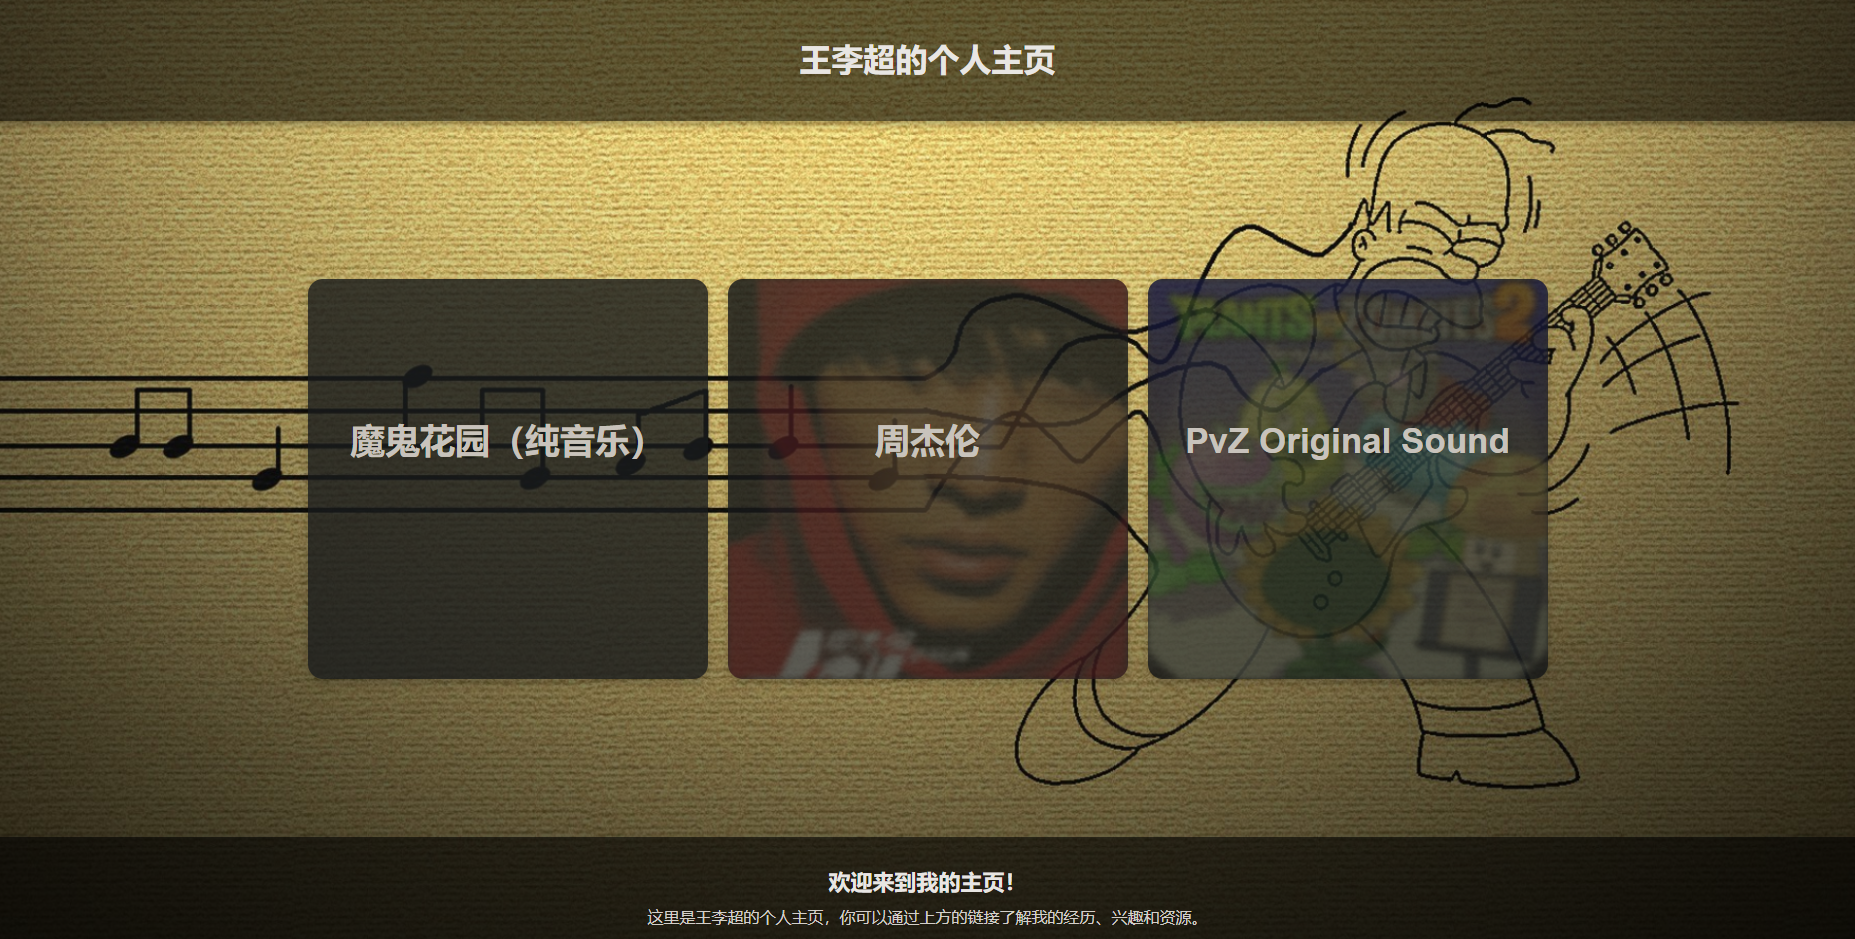
\includegraphics[scale=0.30]{images/3-2.png}
		\caption{分页面举例}
		\label{fig3-2}
	\end{center}
\end{figure}

以下是与主页面设计有所不同的部分
\begin{shaded*}
	\begin{alg}{不同的部分}
		\label{alg:1}
		\begin{algorithmic}
			\State \ \ \ \ \ \ \ \ \ \ \ \ \textbf{width: 400px;  height: 400px; }
			\State \ \ \ \ \ \ \ \ \ \ \ \ \textbf{opacity: 0.2; /* 默认虚化 */}
			\State \ \ \ \ \ \ \ \ \ \ \ \ \textbf{filter: blur(3px); /* 默认添加模糊效果 */}
		\end{algorithmic}
	\end{alg}
	\end{shaded*}

\subsection{我的steam主页}

图\ref{fig3-3}这个页面是直接保存的页面,没有做修改,主要是为了防止此页面直接跳转时无法正常显示页面背景没有做过多替换,在此就不放出源代码了。

\begin{figure}[htb]
	\begin{center}
		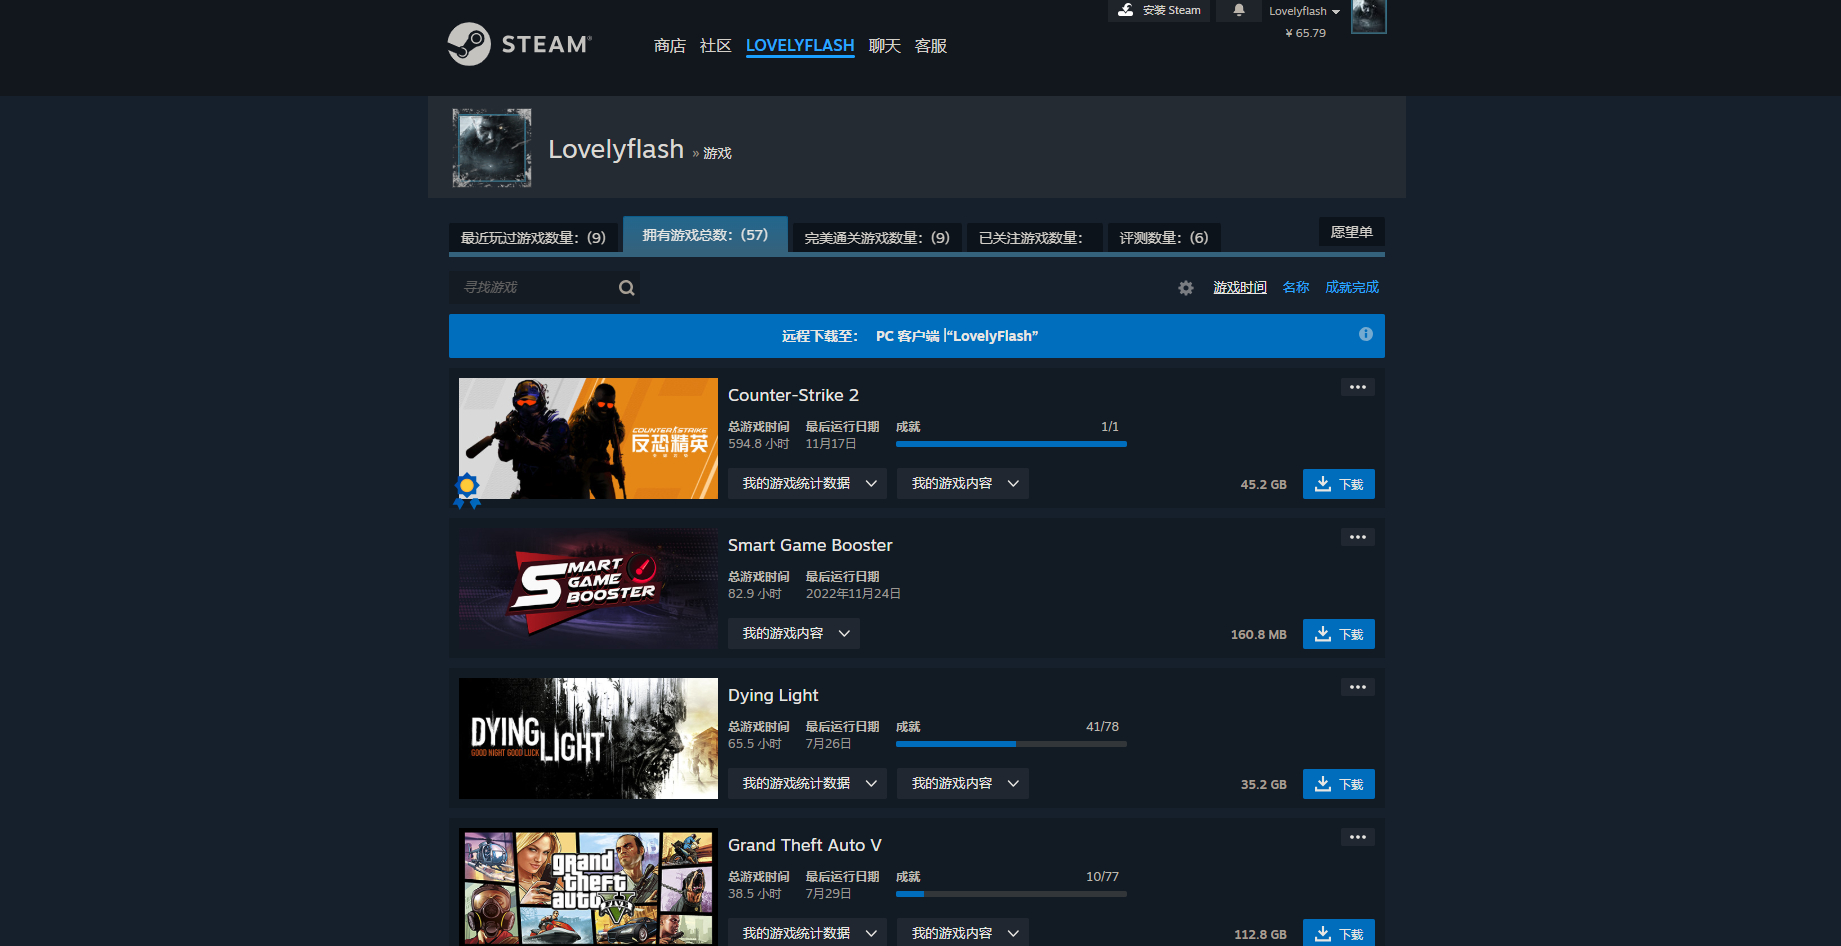
\includegraphics[scale=0.30]{images/3-3.png}
		\caption{分页面举例}
		\label{fig3-3}
	\end{center}
\end{figure}

\subsection{我的GitHub主页}

图\ref{fig3-4}此页面与第一个页面功能有些许重复,但主要是为了提供一个对我现在所写的一个项目的介绍。

\begin{figure}[htb]
	\begin{center}
		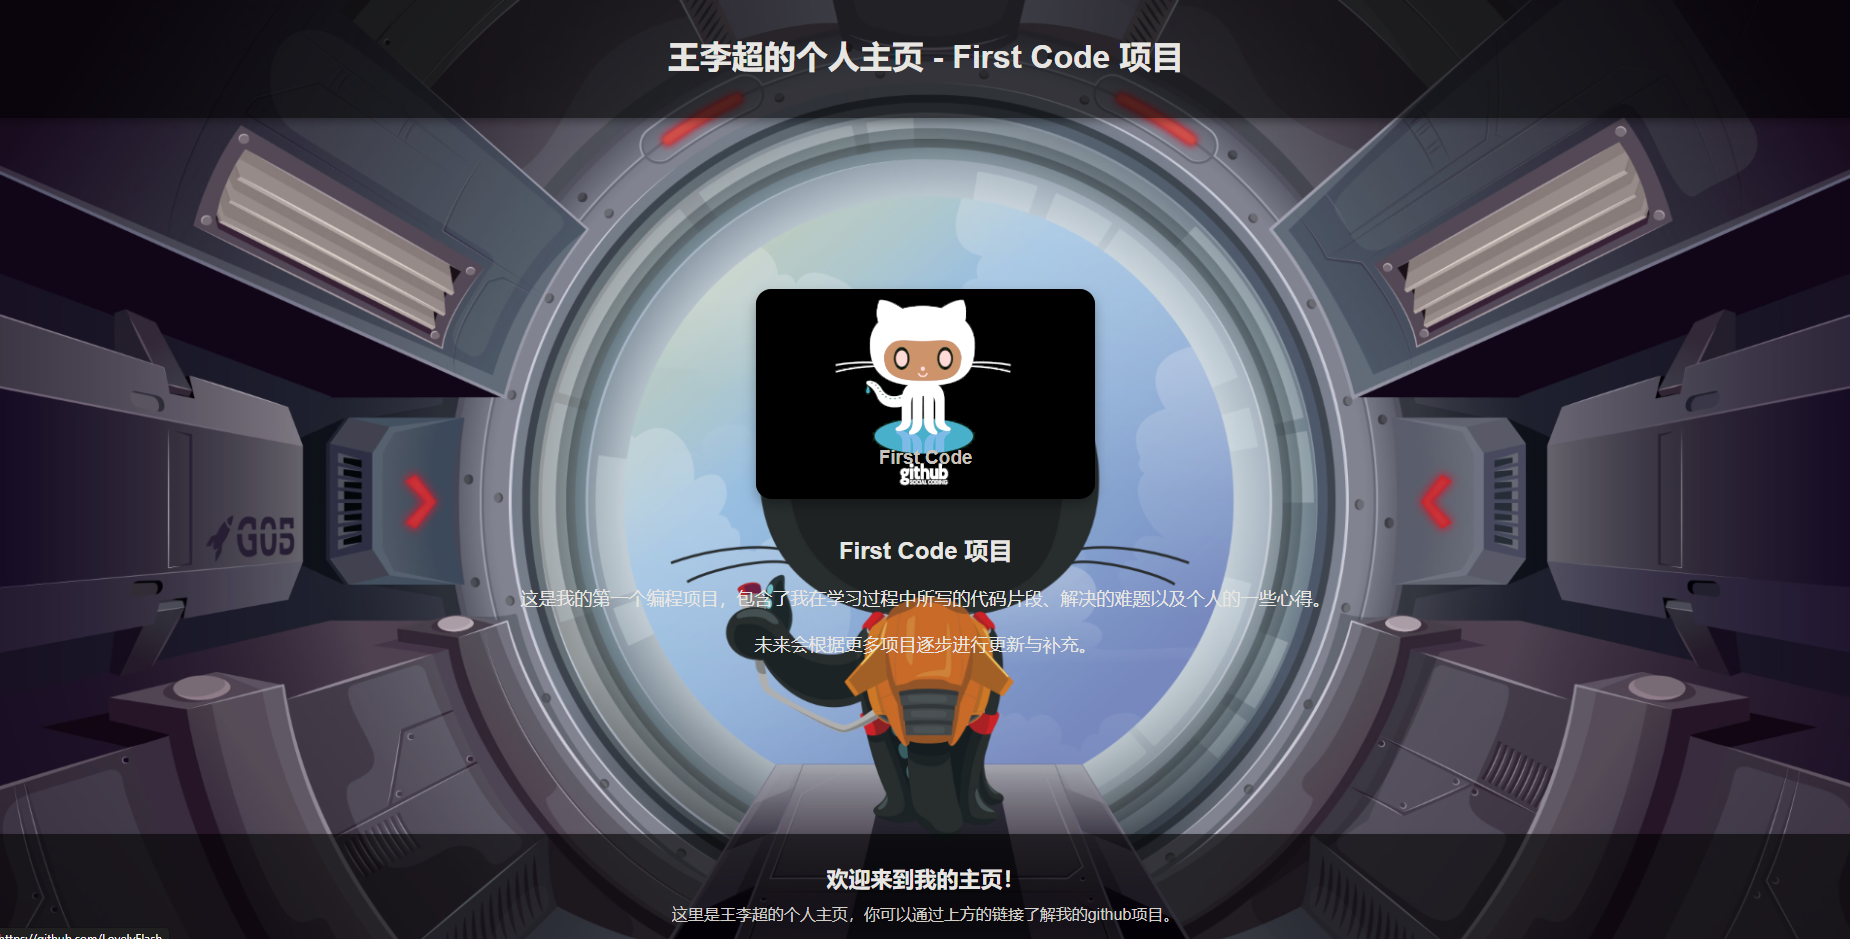
\includegraphics[scale=0.25]{images/3-4.png}
		\caption{分页面举例}
		\label{fig3-4}
	\end{center}
\end{figure}

部分源代码如下

\begin{shaded*}
	\begin{alg}{不同的部分}
		\label{alg:1}
		\begin{algorithmic}
			\State \ \ \ \ \ \ \ \ \ \ \ \ \textbf{width: 400px;  height: 400px; }
			\State \ \ \ \ \ \ \ \ \ \ \ \ \textbf{opacity: 0.2; /* 默认虚化 */}
			\State \ \ \ \ \ \ \ \ \ \ \ \ \textbf{filter: blur(3px); /* 默认添加模糊效果 */}
		\end{algorithmic}
	\end{alg}
	\end{shaded*}

\subsection{我的资源小站}

图\ref{fig3-5}此页面提供了我常用的几个资源小站,在这个页面中首次尝试了JavaScript代码,以显示鼠标悬停时的悬浮显示效果,既与前几个页面风格保持一致,同时对每个方框内的资源做了简要介绍。

部分源代码如下

\begin{shaded*}
	\begin{alg}{不同的部分}
		\label{alg:1}
		\begin{algorithmic}
			\State \textbf{当页面加载完成时,执行以下操作:}
			\State \ \ \ \ \ 创建一个空的工具提示框 (tooltip)
			\State \ \ \ \ \ 将工具提示框添加到文档的主体
			\State \ \ \ \ \ 对每个 .link-box 元素执行以下操作:
			\State \ \ \ \ \ \ \ \ \ 在鼠标进入时,设置工具提示框的文本为元素的 data-description 属性
			\State \ \ \ \ \ \ \ \ \ 设置工具提示框的透明度为 1
			\State \ \ \ \ \ \ \ \ \ 在鼠标移动时,更新工具提示框的位置
			\State \ \ \ \ \ \ \ \ \ 在鼠标离开时,将工具提示框的透明度设置为 0
		\end{algorithmic}
	\end{alg}
\end{shaded*}



\begin{figure}[htb]
	\begin{center}
		
\includegraphics[scale=0.25]{images/3-5.png}
		\caption{分页面举例}
		\label{fig3-5}
	\end{center}
\end{figure}

\newpage

\section{网页设计小结}

在网页设计与实现过程中,遇到了一些挑战,主要涉及以下几个方面:

1. HTML与CSS布局问题
   问题:初期在实现页面时,尤其是在处理不同元素的布局时,存在元素错位或不对齐的情况。例如,header 和 footer 的布局无法保持一致,或者背景图在不同屏幕尺寸下显示不正常。
   
   解决方法:通过使用 flexbox 布局模型来保证元素的对齐和比例。通过设置 flex-direction: column 和 min-height: 100vh,确保页面元素能够正确响应不同屏幕尺寸。同时,使用 background-size: cover 和 background-position: center 确保背景图能够适应页面大小并居中显示。

2. 背景图片与文字的可读性问题
   问题:背景图片的使用虽然提升了网页的视觉效果,但也使得文字在某些区域的可读性降低,尤其是在背景与文字色调相近时。
   
   解决方法:为文本区域添加半透明的背景色(如 rgba(0, 0, 0, 0.6)),同时确保文字颜色为浅色(如白色)以提高对比度,使文字更清晰可读。

3. 标签与内容格式的统一性
   问题:HTML 中标签的使用及其嵌套层级有时难以统一,导致结构复杂或难以维护。例如,多个 div 元素的嵌套层级可能让代码变得冗长。
   
   解决方法:通过精简标签结构,尽量避免多余的嵌套,同时采用语义化标签(如 <header>、<footer>、<main>)提升可读性和可维护性。

4. 网页代码展示问题
   问题:将 HTML 代码转换为伪代码时,如何保持正确的格式和排版,并且确保代码在 LaTeX 环境下能够正确显示,并保持易于理解的结构。
   
   解决方法:使用 algorithmic 环境中的 \State 命令将 HTML 标签和属性逐行列出,并使用 \textbf{} 和 \texttt{} 来格式化标签和CSS样式,确保代码清晰易读,同时通过 shaded* 环境来增强可视化效果。

5. 网页交互性问题
   问题:网页初期设计中缺少交互性,例如用户点击某些链接时没有反馈,或是网页内容未能根据用户输入进行更新。
   
   解决方法:虽然问题没有在设计中显现,但可以通过加入简单的JavaScript或CSS交互效果(如悬停效果、按钮点击响应)来增强用户体验。

6. 图片与其他资源的管理
   问题:在设计时,如何正确引用本地资源(如背景图、图标等)以及如何确保网页在不同设备上的加载表现一致。
   
   解决方法:使用相对路径来引用资源,并确保所有资源文件(如图像、字体文件等)放置在正确的文件夹中。同时,使用合适的格式和大小,确保页面加载速度。

7. 响应式设计
   问题:如何确保网页在不同尺寸的设备上都能正确显示,尤其是在手机、平板和电脑之间切换时。
   
   解决方法:使用 CSS 媒体查询 (@media) 来定义不同设备上的样式规则,确保网页能够根据设备屏幕大小自动调整布局。

8. LaTeX与HTML代码的结合
   问题:如何将 HTML 代码转换为 LaTeX 的伪代码形式,以便在文档中展示。尤其是确保代码在 LaTeX 渲染过程中能保持其原始格式。
   
   解决方法:使用 algorithmic 和 shaded* 环境,在 LaTeX 中逐行描述 HTML 代码的结构,并通过合适的 LaTeX 命令(如 \textbf{} 和 \texttt{})来保持HTML标签和属性的清晰呈现。

\newpage

\section{课程的收获和建议}

通过学习该专题,我初步掌握了HTML设计与制作的几个环节,特别是对一个HTML文件内包含的各个部分有了清晰的认知。在设计网页的过程中,充分体现了理科生的艺术认知,同时保持整体简洁大方。在制作网页的过程中,我充分认识到了“发现问题,分析问题,解决问题”这三步骤对制作过程的重大意义,学会了独立解决问题,也学会了合理使用AI工具,为以后独自完成更复杂网页设计打下坚实基础。

\subsection{计算机基础知识}

通过学习计算机基础知识专题,我对计算机的组成、工作原理和运作机制有了更深的理解。首先,掌握了计算机硬件和软件的基本概念,如中央处理器(CPU)、内存、存储设备等,它们如何协同工作完成复杂任务。其次,学习了操作系统的基本功能,如进程管理、内存管理和文件系统,了解了操作系统如何调度资源,确保系统稳定运行。 

此外,编程语言的基础知识也是关键内容之一,学习了数据结构和算法的基本原理,能够更好地理解如何组织和处理数据,提高编程效率和程序性能。通过实际的编程练习,熟悉了常见的编程语言(如C语言),并理解了如何实现算法设计和数据存储。

通过这些知识的学习,我增强了解决计算机问题的能力,能够从更高层次去分析和理解计算机系统的工作原理,为日后深入学习更复杂的计算机科学课程打下了坚实的基础。

\subsection{文档撰写工具LaTeX}

通过学习文档撰写工具LaTeX专题,我掌握了如何使用LaTeX高效地排版和编写学术性文档。首先,了解了LaTeX的基本语法和结构,学会了如何创建文档、设置章节、插入数学公式、表格和图形等。特别是在处理复杂的数学公式时,LaTeX的强大功能使得表达更加清晰规范。 

其次,学习了如何利用LaTeX生成参考文献、引用和文献管理,这对撰写学术论文或技术文档尤为重要。此外,我还学会了如何使用模板和定制化的样式,快速生成符合学术标准的论文或报告,极大提高了文档制作的效率。

通过实践,掌握了LaTeX的排版优势,使我能够轻松应对格式复杂的文档撰写任务,提升了我的文档编辑能力,为未来的学术研究和论文写作奠定了坚实的基础。

\subsection{编程工具Python}

通过学习Python的基础部分,我掌握了基本语法和常用的数据类型,如字符串、列表、字典、元组等,理解了变量、运算符、条件语句和循环语句的使用。此外,我学习了如何定义函数和处理基本的输入输出。这些基础知识帮助我打下了良好的编程基础,能够编写简单的程序,并为进一步深入学习Python提供了基础。

\subsection{图像设计软件Photoshop}

通过学习图像设计软件Photoshop基础部分,我掌握了图像编辑的基本工具和功能。首先,我学会了如何使用选择工具、画笔工具、涂鸦工具等进行简单的图片修改和修复。其次,了解了图层的概念,学会了如何通过图层管理来独立处理图片中的不同部分。

我还学到了如何调整图像的亮度、对比度和颜色,以优化图片效果。此外,学会了如何添加文字、使用简单的滤镜和特效,进行图像创意设计。这些基础知识使我能够进行日常的图像处理和简单的设计工作,为进一步深入学习Photoshop奠定了基础。

\subsection{版本管理软件Git}

通过学习版本管理软件Git基础部分,我掌握了Git的基本操作和概念。首先,我了解了Git的工作原理,如仓库、分支、提交等基本概念,学会了如何创建本地和远程仓库。通过实践,我掌握了如何使用常见的Git命令,如`git init`、`git add`、`git commit`、`git push`和`git pull`等,能够进行代码版本管理和协作。

此外,我学习了如何使用分支进行代码的独立开发,避免了不同功能的冲突,并学会了如何合并分支。Git的这些基础功能帮助我更好地管理和追踪代码的历史变化,提高了代码协作和团队合作的效率。

\subsection{网页制作Dreamweaver}

通过学习网页制作工具Dreamweaver基础部分,我掌握了网页设计和开发的基本技能。首先,我学会了如何使用Dreamweaver的界面进行网页创建、布局和排版,能够轻松地编辑HTML和CSS代码。通过可视化设计功能,我还学到了如何使用拖放工具快速添加文本、图片和按钮等元素。

此外,我了解了如何进行网页预览和调试,确保网页在不同设备和浏览器上显示正确。Dreamweaver的代码提示和自动完成功能帮助我提高了编程效率,并减少了错误的发生。我还学到了如何组织网页项目文件,管理文件结构。总的来说,这些基础技能为我后续深入学习网页开发和设计提供了坚实的基础。


\nocite{*} %% 作用是不对文献进行引用,但可以生成文献列表

%\bibliographystyle{HustGraduPaper}
%\bibliography{HustGraduPaper}

\end{document}
